\documentclass[10pt]{article}
\usepackage{amsmath}
\usepackage{amssymb}
\usepackage[dvips]{graphicx}
%\usepackage[small,bf]{caption}
%\usepackage[american]{varioref}
%\usepackage{fancyheadings}
%\usepackage{wrapfig}
%\usepackage{html}
%\usepackage{color}
\usepackage{longtable}
% Margin adjustments.  vmargin.sty interacts badly with page numbers at
% the bottom of the page, so we just code the number manually here.

\oddsidemargin  0pt
\evensidemargin 0pt
\topmargin      0pt
\hoffset        0 in
\textwidth      6.5 in
\textheight     9 in

% Style adjustments.

% Fix placement of figures & tables.  This keeps latex from shoving big
% floats to the end of a document when they are somewhat big, which it will
% do even if you put [htb] as the argument.

\setcounter{topnumber}{1}
\setcounter{bottomnumber}{1}
\def\topfraction{1.0}
\def\bottomfraction{1.0}
\def\textfraction{0.0}
\def\floatpagefraction{0.9}

\renewcommand{\arraystretch}{2}

%begin{latexonly}

\raggedbottom

\def\captionfont{\itshape}              % Use italic font for captions.

\makeatletter

\setlength{\parindent}{0 pt}            % Unindented paragraphs, separated ...
\setlength{\parskip}{1.3 ex}            % ... by roughly one blank line.

\renewcommand{\section}{\@startsection%
  {section}{1}{0pt}{-1.8ex \@plus -1ex \@minus -.2ex}%
  {0.8ex}{\normalfont\Large\bfseries}}

\renewcommand{\subsection}{\@startsection%
  {subsection}{2}{0pt}{-2ex \@plus 1ex \@minus -.2ex}%
  {0.8ex}{\slshape\large\bfseries}}

\renewcommand{\subsubsection}{\@startsection%
  {subsubsection}{3}{0pt}{-1.5ex \@plus 1ex \@minus -.2ex}%
  {0.5ex}{\slshape\normalsize\bfseries}}

\newcommand{\tightspacing}{\renewcommand{\baselinestretch}{0.85}}
\newcommand{\regularspacing}{\renewcommand{\baselinestretch}{1.0}}

\newcommand{\bN}{\mbox{\boldmath $N$}}
\newcommand{\bZero}{\mbox{\boldmath $0$}}
\newcommand{\bLo}{\mbox{\boldmath $L_0$}}
\newcommand{\bNo}{\mbox{\boldmath $N_0$}}
\newcommand{\bNr}{\mbox{\boldmath $N_R$}}
\newcommand{\D}{\displaystyle}

\makeatother

% Page footings.

%\pagestyle{fancy}
%\setlength{\headrulewidth}{0 pt}
%\lhead{} \chead{} \rhead{}
% \lfoot{\emph{Internal design document}}
% \rfoot{\emph{Do not quote or redistribute}}

%end{latexonly}

% Miscellaneous macros.

\newcommand{\boxedgraphic}[2][]{\def\fboxsep{0pt}\fbox{\includegraphics[#1]{#2}}}
\newcommand{\url}[1]{\textup{\texttt{#1}}}
\newcommand{\menu}[1]{\textsf{\textbf{#1}}}
\newcommand{\class}[1]{\textsf{#1}}
\newcommand{\attrib}[1]{\textsf{#1}}
\newcommand{\attribtype}[1]{\textsf{#1}}

\newcommand{\notationdocloc}{\url{ftp://ftp.cds.caltech.edu/pub/caltech-erato/notation/}}
\newcommand{\eratowebloc}{\url{http://www.cds.caltech.edu/erato/}}

\begin{document}

%=============================================================================
% Title page
%=============================================================================

%\thispagestyle{fancy}

\title{\textbf{An XML-Based Model Description Language\\
    for Systems Biology Simulations}}

\author{Andrew Finney, Herbert Sauro, Michael Hucka, Hamid Bolouri\\
\normalsize\texttt{\{mhucka,hsauro,afinney,hbolouri\}@cds.caltech.edu}\\[-2pt]
\normalsize ERATO Kitano Systems Biology Project\\[-2pt]
\normalsize Control and Dynamical Systems 107-81\\[-2pt]
\normalsize California Institute of Technology, Pasadena, CA 91125\\[10pt]
\normalsize This document is based on discussions with the authors of\\[-2pt]
\normalsize BioSpice (Arkin), DBSolve (Goryanin), E-Cell (Tomita, Nakayama, Takahashi),\\[-2pt]
\normalsize Gepasi (Mendez), StochSim (Bray, Firth \& Shimizu), Virtual Cell (Loew \& Schaff),\\[-2pt]
\normalsize and the ERATO Kitano Systems Biology Project group.}

\date{\today{}}

\maketitle

\vspace*{0.5 in}

%=============================================================================
\section{Introduction}
\label{sec:introduction}
%=============================================================================

We present a first attempt at specifying a common, model-based
description language for systems biology simulation software,
which we tentatively call the \underline{S}ystem
\underline{B}iology \underline{M}arkup \underline{L}anguage
(SBML). The overall goal is to develop a common language that
will enable simulation software to communicate and exchange
models, ultimately leading to the ability for researchers to run
simulations and analyses across multiple software packages.

SBML is the result of merging the most obvious modeling-language
features of BioSpice, E-Cell, Gepasi, DBSolve, StochSim, Jarnac,
and Virtual Cell.  The description language is encoded in XML, the
Extensible Markup Language~(Bosak and Bray, 1999; Bray, Paoli and
Sperberg-McQueen, 1998).  This XML encoding of the description
language defines a file format; however, at this time, we are
focusing on using the XML-based description language as an
interchange format for use in communications between programs.

The primary purpose of this document is to serve as a basis for
discussion and further development of a more comprehensive
language specification. The final outcome of this process will be
an XML Schema which can be used to communicate model descriptions
between simulation packages. Appendix \ref{apdx:schemas} contains
the most recent version of this schema.  As XML Schemas are
difficult to read and absorb by human readers, we define the
proposed data structures using a succinct graphical notation
based on a subset of UML, the Unified Modeling Language
(Eriksson, 1998; Oestereich, 1999).  Our notation is explained in
\emph{A Notation for
  Describing Model Representations Intended for XML Encoding}~(Hucka,
2000), available online at \notationdocloc{}.  For the sake of clarity, we
ask readers to use this notation when contributing to discussions about the
specification.  To facilitate discussions, a web/FTP site and a group
mailing list have been set up for the seven participating groups.  Please
see the web site at \eratowebloc{} for details.

A few assumptions about the form of the language are not
necessarily self-evident.  In particular,
\begin{itemize}

\item We assume that, in order for each simulator program to read and write
  the model description language, it will require native interface code or
  some stream/file converter.
  This interface code will have to translate the simulator's internal data
  structures back and forth from the model description language.  We assume
  that this interface code will massage data structures as appropriate in
  order to smooth out small differences in conceptual organization between
  a simulator's specific internal representation and the model description
  language.

\item A zero value is not the same as an empty attribute value.  The model
  description language uses a number of structures that, in a given object
  instance, may be empty, depending on whether a given simulator needs
  them.  Programs that interpret objects expressed in the language must be
  designed to pay attention to this distinction.

\end{itemize}

In the XML schema elements names start with a lowercase letter
and defined types or classes start with a uppercase letter being
consistent with ~(Hucka, 2000). In the following text class and
elements are emphasized.  For example \class{Compartment} is a
class name and \class{compartment} is an element name.

Appendix \ref{sec:xml-rep} contains several examples of models encoded in XML.
The following text quotes sections of XML from these models.

%=============================================================================
\section{Overview}
\label{sec:overview}
%=============================================================================

The representation language is organized around five categories of
information: model, compartment, geometry, specie and reaction.
Not all of these will be needed by every simulation package;
rather, the intent is to cover the range of data structures
needed by the collection of all six simulators examined so far.

\begin{figure}
  \centering
  \includegraphics[scale = 0.75]{top-level.eps}
  \caption{A diagram of the highest level of the object class hierarchy.}
  \label{fig:top-level}
\end{figure}

Figure~\ref{fig:top-level} depicts the highest level of
organization of the objects in the model description language. It
shows that all classes are derived directly or indirectly from the
\class{Identified} class.  \class{Identified} contains attributes
\attrib{ID} of type IDREF and of type string, and elements
\attrib{comment} and \attrib{annotation}.  Two classes are
derived directly from \class{Identified}: \class{Named} and
\class{Anonymous}. Both have the attribute \attrib{name}, of type
name, which is optional on \class{Anonymous} and mandatory on
\class{Named}. The \class{Name} type is a XML simple type
derived from string which has the pattern, in BNF
(Backus-Naur Form):

\begin{verbatim}
Letter ::= 'a'..'z','A'..'Z'
Digit ::= '0'..'9'
Name ::= Letter | '_' { Letter | '_' | Digit}
\end{verbatim}

\attrib{notes} contains XHTML and is intended to store notes
meant to be presented to humans, whereas the \attrib{annotation},
which can contain arbitrary elements, is intended to store
information not necessarily intended for human consumption.

In the following diagrams the attributes on \class{Name} and
\class{Anonymous} are not shown even though they are available on
those classes.

%=============================================================================
\section{Elements of the Model Description Language}
\label{sec:elements}
%=============================================================================

In the following sections, we discuss in turn each of the major
classes that are derived from \class{Named} or \class{Anonymous}
in the representational hierarchy.


%-----------------------------------------------------------------------------
\subsection{Model}
%-----------------------------------------------------------------------------

The \class{Model} class defines a grouping of components i.e. a
model does not necessarily model a single specific biological
entity.  There is only one element of type \class{Model} per
instance of a model description language document or data stream,
and it contains the list of compartments, species and reactions
that define a given model.  The UML-based definition of the class
is shown in Figure~\ref{fig:model}.

\begin{figure}[h]
  \centering
  \includegraphics[scale = 0.75]{model.eps}
  \caption{A diagram of \class{Model}.}
  \label{fig:model}
\end{figure}

The definition shows that there must be at least one specie, one reaction
and one compartment in a model; otherwise, there would be little point in
defining the model in the first place
(subsection \ref{subsection:minimaleg} contains an example of a minimal model).
There is no restriction on the total number of these elements.

In addition a model can consist of zero or more \class{Geometry}, \class{Mapping},
\class{Parameter} and \class{Rule} elements.

Skeletal Example:

\begin{small}
\tightspacing
\begin{verbatim}

<sbml version="1">
    <model>
        <listOfCompartments>
        </listOfCompartments>

        <listOfSpecies>
        </listOfSpecies>

        <listOfReactions>
        </listOfReactions>
    </model>
</sbml>

\end{verbatim}
\regularspacing
\end{small}


%--------------------------------------------------------------------------
\subsubsection{Units}
%---------------------------------------------------------------------------

\class{Model} and other classes have attributes for defining the
units used in the model.  An example of an XML encoded model which
uses this feature is given in subsection \ref{subsection:unitseg}.

SMBL has several `built-in' quantity
types: time, amount of substance, volume and length.  Apart from
amount of substance these are all restricted to metric units
however in all cases the scale of the value given can be modified
via an optional integer attribute representing the power of 10
that the quantity is multiplied by.  Amount of substance can be
expressed in number of molecules depending on the state of the
\attrib{substanceIsNumberOfMolecules} boolean attribute.  Table~\ref{tab:builtin} lists the built-in quantity types and
their associated scale attributes:

\begin{table}[h]
\begin{tabular}{|l|l|l|l|l|}
  \hline
  type & scale attribute name & metric unit & default scale & elements attribute occurs on \\ \hline

  substance & substanceScale & Moles or number of molecules & 1 & \class{Model}, \class{Specie}, \class{KineticLaw} \\
  time & timeScale & Seconds & 1 & \class{Model}, \class{KineticLaw} \\
  volume & volumeScale & litres & 1 & \class{Model} \\
  length & lengthScale & metres & $10^{-6}$ $(\mu)$ & \class{Model}, \class{Geometry}
  \\ \hline

\end{tabular}
\caption{A table of the built-in quantities in SBML}

\label{tab:builtin}
\end{table}

The attributes on \class{KineticLaw}, \class{Specie} and
\class{Geometry} override those on \class{Model}. In various
sections below these units are combined to define the units
involved in formulae.

%This definition shows that \class{Model} in this framework
%is a hierarchical grouping construct.  It does not have geometry or other
%characteristics itself; instead, the \class{Compartment} objects are the
%ones that hold geometries and other attributes.  Compartment objects are
%intented to be the leaf elements in a hierarchical tree, as shown in the
%following illustration, in which the top-most \class{Model}
%object contains two \class{Compartment} objects and another
%\class{Model} object:

%\begin{center}
%  \includegraphics{structure-tree.eps}
%\end{center}

%-----------------------------------------------------------------------------
\subsection{Compartments}
%-----------------------------------------------------------------------------

A \class{compartment} represents a bounded container in which
species are located. The definition of \class{Compartment} is
shown in Figure~\ref{fig:compartment}.

\begin{figure}[h]
  \centering
  \includegraphics[scale = 0.75]{compartment.eps}
  \caption{The \class{Compartment} object class definition.}
  \label{fig:compartment}
\end{figure}

The geometric characteristics of a compartment are described
using a \class{geometry} element and a \class{mapping} element.
The geometry information is optional, allowing compartments to
serve simply as topological structures if desired.

For convenience a compartment has the float attribute
\attrib{volume} which is the total volume of the compartment in
volume units as defined on the \class{model}.  This enables
concentrations of specie to be calculated in the absence of
geometry elements.  Any geometry element associated with the
compartment then overloads this value.

The volume attribute is optional and defaults to 1.

The following is an example of a \class{compartment} element.

\begin{small}
\tightspacing
\begin{verbatim}
<compartment name="cell" volume="1"/>
\end{verbatim}
\regularspacing
\end{small}

Lists of compartments are enumerated within {\tt listOfCompartements},
as in the following example:

\begin{small}
\tightspacing
\begin{verbatim}
<listOfCompartments>
  <compartment name="cytosol" volume="1"/>
  <compartment name="mitochondria" volume="0.3"/>
</listOfCompartments>
\end{verbatim}
\regularspacing
\end{small}


%-----------------------------------------------------------------------------
\subsection{Geometry}
%-----------------------------------------------------------------------------

A \class{model} element can contain zero or more \class{geometry}
elements. The \class{Geometry} class is intended to provide a
means for specifying morphological characteristics of
compartments in simulations.  It is defined in
Figure~\ref{fig:geometry}.

\begin{figure}[h]
  \centering
  \includegraphics[scale = 0.75]{geometry.eps}
  \caption{The \class{Geometry} object class definition.}
  \label{fig:geometry}
\end{figure}

The dimensionality of a compartment can be one, two, or three
dimensions, and a given compartment can have an overall physical
size; these aspects are determined in an instance of a
\class{geometry} element by which of the three size attributes are
given a value: either \attrib{length} (for 1D),
\attrib{surfaceArea} (for 2D), or \attrib{volume} (for 3D).  Some
examples of different dimensionalities are: DNA stretch (1D);
disks in photoreceptors (2D); patch of membrane (2D); cell
nucleus (3D); and dendritic spines (3D).  The size of a
compartment may change over the course of a simulation.

The geometrical information is a boundary specification which can
take the form of a set of $(x,y)$ coordinates (\class{point}
elements) in a global reference frame.  The lists are contained
by the attributes \attrib{formulas} and \attrib{coordinates},
respectively.

All the values on a \class{geometry} elements and its associated
elements are in length units as defined on the \class{geometry}
element.  If these units are not defined on the \class{geometry}
element the definition on the \class{model} element is used
instead.

%-----------------------------------------------------------------------------
\subsection{Mapping}
%-----------------------------------------------------------------------------
A \class{model} element can contain zero or more \class{mapping}
elements.  A \class{mapping} element maps a \class{compartment}
element to a \class{geometry} element.  Thus \class{Mapping} has
two name attributes \attrib{compartment} and \attrib{geometry}.
\class{Mapping} is defined in Figure~\ref{fig:mapping}.

\begin{figure}[h]
  \centering
  \includegraphics[scale = 0.75]{mapping.eps}
  \caption{The \class{Mapping} object class definition.}
  \label{fig:mapping}
\end{figure}


%-----------------------------------------------------------------------------
\subsection{Species}
%-----------------------------------------------------------------------------

``Species'' comprise all entities which take part in reactions.  The
\class{Specie} class is intended to represent these entities.  These
include simple ions (e.g., protons, calcium, etc.), simple molecules (e.g.,
glucose, ATP, etc.), and large molecules (e.g., RNA, polysaccharides, and
proteins).  Figure~\ref{fig:specie} presents the definition of
\class{Specie}.

\begin{figure}[h]
  \centering
  \includegraphics[scale = 0.75]{specie.eps}
  \caption{The \class{Specie} object class definition.}
  \label{fig:specie}
\end{figure}

The attribute \attrib{initialAmount}, of type float, is used to
set the initial amount of the specie.  These are in the substance
units as defined on \class{Specie} via the
\attrib{substanceScale} and \attrib{substanceIsNumberOfMolecules}
attributes in the way described in the Model section above.  If
these units are not defined on a \class{Specie} element the
definition on the \class{Model} element is used instead.

The boolean attribute \attrib{boundaryCondition} determines
whether the amount of the specie is fixed or variable over the
course of a simulation. \attrib{boundaryCondition} is optional
and defaults to false. The attribute \attrib{compartment}, of
type name, is used to identify the compartment in which the
specie belongs.

The integer attribute \attrib{charge} indicates the charge on the
species (in terms of electrons not the SI unit Coulombs).

The following is an example of a minimal \class{specie} element.

\begin{small}
\tightspacing
\begin{verbatim}
<specie name="s1" compartment="cell" initialAmount="4"/>
\end{verbatim}
\regularspacing
\end{small}

Lists of species are enumerated within {\tt listOfSpecies},
as in the following example:

\begin{small}
\tightspacing
\begin{verbatim}
<listOfSpecies>
  <specie name="Glucose" compartment="cell" initialAmount="4"/>
  <specie name="Glucose_6_P" compartment="cell" initialAmount="4"/>
  ...
</listOfSpecies>
\end{verbatim}
\regularspacing
\end{small}


%-----------------------------------------------------------------------------
\subsection{Parameters}
%-----------------------------------------------------------------------------

A \class{parameter} element associates a symbol with a float value
so that the symbol can be used in formulae instead of the value.
The \class{Parameter} class is defined in
figure~\ref{fig:parameter}. The symbol is taken from the
\attrib{name} attribute and the value is taken from the
\attrib{value} attribute.  A parameter can be associated with a
model or a reaction.  The parameter elements associated with the
model define parameters that are {\em global} to the whole model.
The parameter elements associated with a reaction {\em overload}
global parameters (see subsection \ref{subsection:namespace} for
further details).

\begin{figure}[h]
  \centering
  \includegraphics[scale = 0.75]{parameter.eps}
  \caption{The \class{Parameter} object class definition.}
  \label{fig:parameter}
\end{figure}

The following is an example of a simple \class{parameter} element.
\begin{small}
\tightspacing
\begin{verbatim}
<parameter name="k1" value="1.2"/>
\end{verbatim}
\regularspacing
\end{small}

The \class{Parameter} class has an integer attribute
\attrib{scale} and a name attribute \attrib{unit} for annotating
the unit type of the parameter.  Both these attributes are
optional.  As for the built in types the \attrib{scale} attribute
is a power of ten multiplier and the \attrib{unit} is an
arbitrary symbol for any type.

The following is an example of a \class{parameter} element which defines a symbol,
$Vm$ , to be $3\ mM\ l^{-1}\ s^{-1}$.
\begin{small}
\tightspacing
\begin{verbatim}
<parameter name="Vm" value="3" scale="-3" unit="molesPerLitrePerSecond"/>
\end{verbatim}
\regularspacing
\end{small}

Lists of parameters are enumerated within {\tt listOfParameters},
as in the following example:

\begin{small}
\tightspacing
\begin{verbatim}
<listOfParameters>
  <specie name="Km1" value="2.3"/>
  <specie name="Km2" value="10.7"/>
  ...
</listOfParameters>
\end{verbatim}
\regularspacing
\end{small}


An example of an XML encoded model which
uses this feature is given in subsection \ref{subsection:unitseg}.

%-----------------------------------------------------------------------------
\subsection{Rules}
%-----------------------------------------------------------------------------
A model can contain a list of \class{rule} elements.

A \class{rule} element represents a formula of the form `x=y'.
Thus a rule has two attributes \attrib{lhs} and \attrib{rhs}.
\attrib{lhs} is a name attribute and contains either a species
name or a new computed parameter name. Computed parameters are
declared by rules.  Computed parameters can be used in formulae.
The \attrib{rhs} attribute contains a formula string.

\class{rule} elements are evaluated in the order given in the XML
stream/file.

Rules are included to enable, for example, the computation of the
equilibrium concentrations of fast reactions and modeling pH.

The following is an example of a \class{rule} element.
\begin{small}
\tightspacing
\begin{verbatim}
      <rule lhs="s2" rhs="k*t/(1+k)"/>
\end{verbatim}
\regularspacing
\end{small}

When the simulation application reads the model specification it
will build a set of ordinary differential equations (ODE), these
will be used by the simulator to perform various analyses on the
model. It is the intention, that the rule expressions be an
integral part of the ODE expression list and must be evaluated
by the simulator just before the ODE list.

An example of an XML encoded model which uses \class{rule} elements is given in
subsection \ref{subsection:ruleseg}.

%-----------------------------------------------------------------------------
\subsection{Formulae}
%-----------------------------------------------------------------------------

Two classes, \class{KineticLaw}, and \class{Rule} have string
attributes which contain formulae, \attrib{formula} and
\attrib{rhs} respectively.  These are interpreted as expressions which
evaluate to a float value. All operators in these expressions return float
values.  For boolean operators, 0 is interpreted as false.  All
other values are interpreted as true.  The operators available in
these expressions are shown in table~\ref{tab:operators}.

\begin{table}[h]
\begin{center}
\begin{tabular}{|l|l|l|l|l|}
\hline
 Tokens & Operator & Class & Precedence & Associates \\
\hline

\emph{names} & names & primary & 8 & n/a \\
(\emph{expression}) & sub expression & primary & 8 & n/a\\
\emph{f}(\emph{...}) & function call & postfix & 8 & left\\
not, ! & logical not & unary & 7 & right\\
- & negation & unary & 6 & right\\
\verb|^| & power & binary & 5 & left \\
* & multiplication & binary & 4 & left\\
/ & division & binary & 4 & left\\
+ & addition & binary & 3 & left\\
- & subtraction & binary & 3 & left\\
and \&\& & logical and & binary & 2 & left\\
or \verb+||+ & logical or & binary & 1 & left\\
xor & logical exclusive or & binary & 1 & left\\
\hline
\end{tabular}
\caption{A table of the expression operators in SBML}
\end{center}
\label{tab:operators}
\end{table}

We are not expecting simulators to support the logical operators
in the near future.

The function call operator consists of a function name followed
by an `(' token followed by a sequence of zero or
more argument expressions separated by commas followed by a `)'
token. Table~\ref{tab:simplemath} in Appendix \ref{appendix:simplemath}
shows the basic math functions that are available.

Table~\ref{tab:ratelaws} in Appendix \ref{appendix:ratelaws}
contains all the built in rate law functions.

In these formulae the name tokens (other than function names) are
the names of either parameters, computed parameters, compartments
or species.  For the purposes of this document we call these
\emph{symbols}.

When a species name occurs in a formula it represents the concentration
($substance/volume$) of the specie. The units of this value are
derived from the \attrib{volumeScale} attribute value on the
\class{model} element and the substance units defined for the
\class{Specie} (see the section on Specie).

When a compartment name
occurs in a formula it represents the volume of the compartment. Again the units of
this value are derived from the \attrib{volumeScale} attribute value on the
\class{model} element.

%-----------------------------------------------------------------------------
\subsection{Namespaces}
\label{subsection:namespace}
%-----------------------------------------------------------------------------

The names of parameter elements contained in a \class{reaction}
element are unique to just the reaction and override parameter
and specie names declared elsewhere i.e. parameter symbols can be defined in one of two names spaces, a local space confined to
particular rate laws and a global space.
The advantage of this is that some simulators currently use a local name space approach when declaring rate laws. This allows them
to use the same symbol (but different instance) in many different rate laws which reduces the burden that the modeller sometimes has
when collating a collection of parameter names. On the other hand, some simulators require the user to generate unique symbol names
for every distinct parameter. To accomodate this approach, we introduced the global name space. In addition the global name space
allows sets of rate equations and rules to share the same parameter symbol (single instance). For example a particular enzyme might
catalyze a number of different reactions in which case it would be an advantage to specific a single parameter indicating the concentration
of enzyme which would appear in all the effected rate laws.

%-----------------------------------------------------------------------------
\subsection{Reactions}
%-----------------------------------------------------------------------------

A \class{reaction} represents some transformation, transport or
binding process, typically a chemical reaction, which can change
the amount of one or more species.  \class{Reaction} is defined
in figure~\ref{fig:reaction}.  In this framework, reactions are
defined using lists of reactant species, products, and their
stoichiometries, and by parameter values for separately-defined
kinetic laws.

\begin{figure}[h]
  \centering
  \includegraphics[scale = 0.75]{reaction.eps}
  \caption{The \class{Reaction} object class definition.}
  \label{fig:reaction}
\end{figure}

\class{Reaction} has a boolean attribute, \attrib{reversible},
which is false by default.

The examples in appendix \ref{sec:xml-rep} clarify how the
elements of the \class{Reaction} class are intended to be used.

%-----------------------------------------------------------------------------
\subsubsection{SpeciesReference}
%-----------------------------------------------------------------------------

An instance of \class{SpeciesReference} links a specie to a
\class{reaction}. This implies that the reaction will affect the
amount of that specie. The attribute \attrib{specie},
of type name, in the \class{SpecieReference} class in
Figure~\ref{fig:reaction} is intended to refer to the name of a
specie in the species list of the model.  In other words, the
species involved in a reaction are listed once in a model and the
\attrib{listOfReactants} and \attrib{listOfProducts} in reactions
refer to the list of species.  The instances of \class{SpeciesReference}
are \class{reactant} and \class{product} elements in the
\attrib{listOfReactants} and \attrib{listOfProducts} respectively.

The following is a simple example of a \class{reactant} element.
\begin{small}
\tightspacing
\begin{verbatim}
<reactant specie="X0" stoichiometry="1"/>
\end{verbatim}
\regularspacing
\end{small}

The effective stoichiometry value is created by dividing the
\attrib{stoichiometry} attribute value by the
\attrib{denominator} attribute value. The attribute
\attrib{stoichiometry} is of type integer and is optional,
defaulting to 1. The attribute \attrib{denominator} is of type
integer and is optional, defaulting to 1. (This allows the user to
employ rational arithmetic computations on the stoichiometry
matrix. This helps to eliminate roundoff errors and other
problems during the computation, especially for large matrices.
These computations are particularly important when calculating
things like elementary modes.)

%-----------------------------------------------------------------------------
\subsubsection{KineticLaw}
%-----------------------------------------------------------------------------

A \class{kineticLaw} element describes the rate of the enclosing
reaction.  The \attrib{formula}, of type string, expresses the
rate in $substance / time$ units. The exact units for substance
and time used can be given via the \attrib{substanceScale},
\attrib{timeScale} and \attrib{substanceIsNumberOfMolecules}
attributes on KineticLaw in the way described in the \class{model}
section above.  These attributes are optional and the default
values are taken from the \class{Model} element.

The \class{kineticLaw} element contained in a \class{reaction}
element is optional however in general there is no default element
that can be substituted in place of a missing \class{kineticLaw}
element.

\class{KineticLaw} contains zero or more \class{parameter}
elements which define symbols that can be used in the formula
string.  These symbols overload those defined at the model level.

The following is a simple example of a \class{kineticLaw} element.
\begin{small}
\tightspacing
\begin{verbatim}
<kineticLaw formula="k1*X0">
    <listOfParameters>
        <parameter name="k1" value="0"/>
    </listOfParameters>
</kineticLaw>
\end{verbatim}
\regularspacing
\end{small}

%-----------------------------------------------------------------------------
\subsubsection{An example of a complete reaction element}
%------------------------------------------------------------------------------

The following is an example of a \class{reaction} element.
\begin{small}
\tightspacing
\begin{verbatim}
<reaction name="J1">
    <listOfReactants>
        <reactant specie="X0" stoichiometry="1"/>
    </listOfReactants>
    <listOfProducts>
        <product specie="S1" stoichiometry="1"/>
    </listOfProducts>
    <kineticLaw formula="k1*X0">
        <listOfParameters>
            <parameter name="k1" value="0"/>
        </listOfParameters>
    </kineticLaw>
</reaction>
\end{verbatim}
\regularspacing
\end{small}

%------------------------------------------------------------------------------
\section{Versions of the markup language}
%------------------------------------------------------------------------------

The top level element \class{sbml} has the integer attribute
\attrib{version} which indicates which version of this standard
that the XML stream/file complies with.

%------------------------------------------
\section{Future Enhancements}
%-------------------------------------------
We currently considering the following features for future
versions of SBML:

%-------------------------------------------
\subsection{Literature References}
%-------------------------------------------
This feature will allow the models to be annotated with
references to papers and authors.


%-------------------------------------------
\subsection{Explicit references to ODEs}
%-------------------------------------------
A model should be able to explicitly specify ordinary differential
equations alongside the rules and reactions. One application of
this would be to allow the modelling of variable volume spaces.

%-------------------------------------------
\subsection{Submodels}
%-------------------------------------------
This feature will allow the reuse of model libraries and the
creation of several instances of the same model.

%-------------------------------------------
\subsection{Indices}
%-------------------------------------------
This feature will allow sets of similar reactions to be defined
which transform sets of species.  A Formula string could then
include `sum' and `product' functions.

%---------------------------------------------
\subsection{DNA}
%-------------------------------------------
This feature will allow DNA to be explicitly modeled.

%-------------------------------------------
\subsection{Diagrams}
%-------------------------------------------
This feature will allow elements to be annotated with data to
enable the display of the model in a diagram.

%=============================================================================
\section{What to Do If You Have Read This Far}
\label{sec:what}
%=============================================================================

Please use the group email address (\texttt{sysbio@caltech.edu})
and web site \eratowebloc{} to send us your comments and
suggestions.

\appendix

%=============================================================================
\section{Using the XML Encoding of the Model Description Language}
\label{sec:xml-rep}
%=============================================================================

In this section, we present an example of translating a model
into the systems biology model description language defined in
this document.  The approach to translating into XML the object
class definitions presented in the sections above is described in
the companion document \emph{A
  Notation for Describing Model Representation Intended for XML
  Encoding}~(Hucka, 2000).  Appendix~\ref{apdx:schemas} gives the full
listing of a preliminary version of an XML Schema corresponding
to the systems biology model description language.

%-----------------------------------------------------------------------------
\subsection{Minimal Model}
%-----------------------------------------------------------------------------
The following model uses the minimum number of elements and attributes possible in SBML.

\begin{small}
\tightspacing
\begin{verbatim}

<sbml version="1">
    <model>
        <listOfCompartments>
            <compartment name="x"/>
        </listOfCompartments>
        <listOfSpecies>
            <specie name="x" compartment="x" initialAmount="1"/>
        </listOfSpecies>
        <listOfReactions>
            <reaction name="x">
                <listOfReactants>
                    <reactant specie="x"/>
                </listOfReactants>
                <listOfProducts>
                    <product specie="x"/>
                </listOfProducts>
            </reaction>
        </listOfReactions>
    </model>
</sbml>

\end{verbatim}
\regularspacing
\end{small}

%-----------------------------------------------------------------------------
\subsection{Simple use of units feature in a model}
\label{subsection:unitseg}
%-----------------------------------------------------------------------------

The following model uses the units features of SBML.  In this
model the \attrib{substanceScale} attribute on the \class{model}
element has the value -3 which defines all qualities of substance
to be defined in $10^{-3}$ mole units or milliMoles.  (This sets
the default units in the model, elements can override this scale
locally).  The \attrib{volumeScale} and \attrib{timeScale}
attributes are not set ensuring that volume is in litres and time
is in seconds.  Thus by default in this model kinetic law
formulae define rates in milliMoles per second and the specie
symbols in them represent concentration values in milliMoles per
litre.  All the \class{specie} elements set the initial amount of
the given specie to 1 milliMole.

The parameters Vm and Km are defined to be in milliMoles per
Litre per Second and milliMolar respectively. This scale
definition is entirely arbitrary and is not linked by SBML to the
built in units described in the previous paragraph.

\begin{small}
\tightspacing
\begin{verbatim}


<sbml version="1">
    <model substanceScale="-3">
        <listOfCompartments>
            <compartment name="cell"/>
        </listOfCompartments>
        <listOfSpecies>
            <specie name="x0" compartment="cell" initialAmount="1"/>
            <specie name="x1" compartment="cell" initialAmount="1"/>
            <specie name="s1" compartment="cell" initialAmount="1"/>
            <specie name="s2" compartment="cell" initialAmount="1"/>
        </listOfSpecies>
        <listOfParameters>
            <parameter name="vm" value="2" scale="-3" unit="molesPerLitrePerSecond"/>
            <parameter name="km" value="3" scale="-3" unit="moles"/>
        </listOfParameters>
        <listOfReactions>
            <reaction name="v1">
                <listOfReactants>
                    <reactant specie="x0"/>
                </listOfReactants>
                <listOfProducts>
                    <product specie="s1"/>
                </listOfProducts>
                <kineticLaw formula="(vm*s1)/(km+s1)"/>
            </reaction>
            <reaction name="v2">
                <listOfReactants>
                    <reactant specie="s1"/>
                </listOfReactants>
                <listOfProducts>
                    <product specie="s2"/>
                </listOfProducts>
                <kineticLaw formula="(vm*s2)/(km+s2)"/>
            </reaction>
            <reaction name="v3">
                <listOfReactants>
                    <reactant specie="s2"/>
                </listOfReactants>
                <listOfProducts>
                    <product specie="x1"/>
                </listOfProducts>
                <kineticLaw formula="(vm*s1)/(km+s1)"/>
            </reaction>
        </listOfReactions>
    </model>
</sbml>
\end{verbatim}
  \regularspacing
\end{small}


%-----------------------------------------------------------------------------
\subsection{A simple example application using rules}
\label{subsection:ruleseg}
%-----------------------------------------------------------------------------

The following model contains the pathway $X_0 \rightarrow S_1
\rightarrow S_2 \rightarrow X_1$, where $S_1 \rightarrow S_2$ is
a fast reaction. The reaction $S_1 \rightarrow S_2$ is not
modeled explicitly; instead, the effect of the reaction is
encapsulated in rules.

\begin{small}
\tightspacing
\begin{verbatim}

<sbml version="1">
  <model>
    <listOfCompartments>
      <compartment name="cell" volume="1"/>
    </listOfCompartments>
    <listOfSpecies>
      <specie name="s1" compartment="cell" initialAmount="4"/>
      <specie name="s2" compartment="cell" initialAmount="2"/>
      <specie name="x0" compartment="cell" initialAmount="1"/>
      <specie name="x1" compartment="cell" initialAmount="0"/>
    </listOfSpecies>
    <listOfParameters>
      <parameter name="k1" value="1.2"/>
      <parameter name="k2" value="1000"/>
      <parameter name="k3" value="3000"/>
      <parameter name="k4" value="4.5"/>
    </listOfParameters>
    <listOfRules>
      <rule lhs="t" rhs="s1 + s2"/>
      <rule lhs="k" rhs="k3/k2"/>
      <rule lhs="s2" rhs="k*t/(1+k)"/>
      <rule lhs="s1" rhs="t-s2"/>
    </listOfRules>
    <listOfReactions>
      <reaction name="j1">
        <listOfReactants>
          <reactant specie="x0"/>
        </listOfReactants>
        <listOfProducts>
          <product specie="s1"/>
        </listOfProducts>
        <kineticLaw formula="k1*x0"/>
      </reaction>
      <reaction name="j3">
        <listOfReactants>
          <reactant specie="s2"/>
        </listOfReactants>
        <listOfProducts>
          <product specie="x1"/>
        </listOfProducts>
        <kineticLaw formula="k4*s2"/>
      </reaction>
    </listOfReactions>
  </model>
</sbml>

\end{verbatim}
  \regularspacing
\end{small}


%-----------------------------------------------------------------------------
\subsection{A simple example application of the Model Description Language}
%-----------------------------------------------------------------------------

The following example is the main portion of an XML document that
describes a simple branch system of the following form:
\[
\begin{array}{ccc}
& {k1 * X0}\\
X0 & \longrightarrow & S1
\end{array}
\]
\[
\begin{array}{ccc}
& {k2 * S1}\\
S1 & \longrightarrow & X1
\end{array}
\]
\[
\begin{array}{ccc}
& {k3 * S1}\\
S1 & \longrightarrow & X2
\end{array}
\]

The following is the XML encoding of the above reaction.

\begin{small}
\tightspacing
\begin{verbatim}
<sbml version="1">
<model id="simplemodel" name="Branch">
    <notes>
        <body xmlns="http://www.w3.org/1999/xhtml">
            <p>Simple branch system.</p>
            <p>The reaction looks like this:</p>
            <p>reaction-1:   X0 -> S1; k1*X0;</p>
            <p>reaction-2:   S1 -> X1; k2*S1;</p>
            <p>reaction-3:   S1 -> X2; k3*S1;</p>
        </body>
    </notes>
    <listOfCompartments>
        <compartment name="compartmentOne" volume="1"/>
    </listOfCompartments>
    <listOfSpecies>
        <specie name="S1" initialAmount="0" compartment="compartmentOne" boundaryCondition="false"/>
        <specie name="X0" initialAmount="0" compartment="compartmentOne" boundaryCondition="true"/>
        <specie name="X1" initialAmount="0" compartment="compartmentOne" boundaryCondition="true"/>
        <specie name="X2" initialAmount="0" compartment="compartmentOne" boundaryCondition="true"/>
    </listOfSpecies>
    <listOfReactions>
        <reaction name="reaction_1" reversible="false">
            <listOfReactants>
                <reactant specie="X0" stoichiometry="1"/>
            </listOfReactants>
            <listOfProducts>
                <product specie="S1" stoichiometry="1"/>
            </listOfProducts>
            <kineticLaw formula="k1*X0">
                <listOfParameters>
                    <parameter name="k1" value="0"/>
                </listOfParameters>
            </kineticLaw>
        </reaction>
        <reaction name="reaction_2" reversible="false">
                <listOfReactants>
                    <reactant specie="S1" stoichiometry="1"/>
                </listOfReactants>
                <listOfProducts>
                    <product specie="X1" stoichiometry="1"/>
                </listOfProducts>
            <kineticLaw formula="k2*S1">
                <listOfParameters>
                        <parameter name="k2" value="0"/>
                </listOfParameters>
            </kineticLaw>
        </reaction>
            <reaction name="reaction_3" reversible="false">
                <listOfReactants>
                    <reactant specie="S1" stoichiometry="1"/>
                </listOfReactants>
                <listOfProducts>
                    <product specie="X2" stoichiometry="1"/>
                </listOfProducts>
                <kineticLaw formula="k3*S1">
                    <listOfParameters>
                        <parameter name="k3" value="0"/>
                    </listOfParameters>
                </kineticLaw>
            </reaction>
        </listOfReactions>
    </model>
</sbml>

\end{verbatim}
  \regularspacing
\end{small}

The corresponding XML encoding shown above is quite
straightforward. The outermost container is a tag, \texttt{smbl},
that identifies the contents as being \underline{s}ystems
\underline{b}iology \underline{m}arkup \underline{l}anguage, an
application of XML. The next-inner container is a single
\texttt{model} element which serves as the highest-level object in
the model.  The model in this case contains a single
\texttt{compartment} element.

The compartment has four species associated with it, and three
reactions. The correspondence between these elements and the
three reaction equations list above should be fairly obvious in
the XML.  The elements in the
\texttt{listOfReactants} and \texttt{listOfProducts} refer to the
names of elements listed in the \texttt{listOfSpecies}.

The lone \texttt{compartment} has no value for \texttt{volume}
because its irrelevant for this particular simple case example.
Since its an optional attribute, there is no mention of it in the
XML object.

Note that the \texttt{comment} elements of the specie and
reaction elements above have been omitted, because they are
empty.  The XML Schema definition in Appendix~\ref{apdx:schemas}
is defined in such a way that the \texttt{name} and
\texttt{comment} fields in the \class{Anonymous} element are
optional.


%=============================================================================
\section{XML Schema for the Model Description Language}
\label{apdx:schemas}
%=============================================================================

The following is a first draft of an XML Schema definition for
the systems biology model description language described above.
Example applications of this XML Schema is presented in
Appendix~\ref{sec:xml-rep}.

The schema below is well formed and compiles with an XML schema schema
however the use of unique and keyref elements in this schema has not been fully
validated.  The other elements have been fully validated.
In practice the unique and keyref elements may either need to be commented out or
will be ignored as they are not supported by most XML parsers.

\begin{small}
\tightspacing
\begin{verbatim}
<schema xmlns="http://www.w3.org/1999/XMLSchema"
        targetNamespace="http://www.cds.caltech.edu/erato/schemas"
        xmlns:sbml="http://www.cds.caltech.edu/erato/schemas/sbml">

    <xsd:annotation>
        <xsd:documentation>
            File name   : sbml.xsd
            Description : XML Schema for the Systems Biology Markup Language
            Organization: Caltech ERATO Kitano
            Version     : 1
            Modified    : 2000-08-07 13:51 PDT
        </xsd:documentation>
    </xsd:annotation>

    <!-- Name -->

    <xsd:simpleType base="xsd:string" name="Name">
        <xsd:pattern value="(_|[a-z]|[A-Z])(_|[a-z]|[A-Z]|[0-9])*"/>
    </xsd:simpleType>

    <!-- Identified -->

    <xsd:complexType name="Identified" abstract="true">
        <xsd:element name="notes" maxOccurs="1" minOccurs="0">
            <xsd:complexType>
                <xsd:any namespace="http://www.w3.org/1999/xhtml" maxOccurs="unbounded" minOccurs="1" processContents="skip"/>
            </xsd:complexType>
        </xsd:element>
        <xsd:element name="annotation" maxOccurs="1" minOccurs="0">
            <xsd:complexType>
                <xsd:any maxOccurs="*" minOccurs="1" processContents="skip"/>
            </xsd:complexType>
        </xsd:element>
        <xsd:attribute name="id" type="xsd:ID" use="optional"/>
    </xsd:complexType>

    <!-- Anonymous-->

    <xsd:complexType name="Anonymous" base="Identified" derivedBy="extension" abstract="true">
        <xsd:attribute name="name" type="Name" use="optional"/>
    </xsd:complexType>

    <!--Named-->
    <xsd:complexType name="Named" base="Identified" derivedBy="extension" abstract="true">
        <xsd:attribute name="name" type="Name" use="required"/>
    </xsd:complexType>

    <!-- listOfParameters -->

    <xsd:element name="listOfParameters">
        <xsd:complexType>
            <xsd:element name="parameter" type="Parameter" minOccurs="1" maxOccurs="unbounded"/>
        </xsd:complexType>
    </xsd:element>

    <!-- Model -->

    <xsd:complexType name="Model" base="Anonymous" derivedBy="extension">
        <xsd:element name="listOfCompartments" minOccurs="1" maxOccurs="1">
            <xsd:complexType>
                <xsd:element name="compartment" type="Compartment" minOccurs="1" maxOccurs="unbounded"/>
            </xsd:complexType>
        </xsd:element>
        <xsd:element name="listOfGeometries" minOccurs="0" maxOccurs="1">
            <xsd:complexType>
                <xsd:element name="geometry" type="Geometry" minOccurs="1" maxOccurs="unbounded"/>
            </xsd:complexType>
        </xsd:element>
        <xsd:element name="listOfMappings" minOccurs="0" maxOccurs="1">
            <xsd:complexType>
                <xsd:element name="mapping" type="Mapping" minOccurs="1" maxOccurs="unbounded"/>
            </xsd:complexType>
        </xsd:element>
        <xsd:element name="listOfSpecies" minOccurs="1" maxOccurs="1">
            <xsd:complexType>
                <xsd:element name="specie" type="Specie" minOccurs="1" maxOccurs="unbounded"/>
            </xsd:complexType>
        </xsd:element>
        <xsd:element ref="listOfParameters" minOccurs="0" maxOccurs="1"/>
        <xsd:element name="listOfRules" minOccurs="0" maxOccurs="1">
            <xsd:complexType>
                <xsd:element name="rule" type="Rule" minOccurs="1" maxOccurs="unbounded"/>
            </xsd:complexType>
        </xsd:element>
        <xsd:element name="listOfReactions" minOccurs="1" maxOccurs="1">
            <xsd:complexType>
                <xsd:element name="reaction" type="Reaction" minOccurs="1" maxOccurs="unbounded">
                    <xsd:unique name="parameters">
                        <xsd:selector>listOfParameters/parameter</xsd:selector>
                        <xsd:field>@name</xsd:field>
                    </xsd:unique>
                </xsd:element>
            </xsd:complexType>
        </xsd:element>
        <xsd:attribute name="substanceScale" type="xsd:integer" use="default" value="0"/>
        <xsd:attribute name="timeScale" type="xsd:integer" use="default" value="0"/>
        <xsd:attribute name="volumeScale" type="xsd:integer" use="default" value="0"/>
        <xsd:attribute name="lengthScale" type="xsd:integer" use="default" value="-6"/>
        <xsd:attribute name="substanceIsNumberOfMolecules" type="xsd:boolean" use="default" value="false"/>
    </xsd:complexType>

    <!-- Compartment -->

    <xsd:complexType name="Compartment" base="Named" derivedBy="extension">
        <xsd:attribute name="volume" type="xsd:float" use="default" value="1"/>
    </xsd:complexType>

    <!-- Geometry -->
    <xsd:complexType name="Geometry" base="Named" derivedBy="extension">
        <xsd:element name="listOfPoints" minOccurs="0" maxOccurs="1">
            <xsd:complexType>
                <xsd:element name="point" type="Point" minOccurs="1" maxOccurs="unbounded"/>
            </xsd:complexType>
        </xsd:element>
        <xsd:attribute name="length" type="xsd:float" use="optional"/>
        <xsd:attribute name="surfaceArea" type="xsd:float" use="optional"/>
        <xsd:attribute name="volume" type="xsd:float" use="optional"/>
        <xsd:attribute name="lengthScale" type="xsd:integer" use="optional"/>
    </xsd:complexType>

    <xsd:complexType name="Point" base="Anonymous" derivedBy="extension">
        <xsd:attribute name="x" type="xsd:float" use="required"/>
        <xsd:attribute name="y" type="xsd:float" use="required"/>
    </xsd:complexType>

    <!--Mapping-->

    <xsd:complexType name="Mapping" base="Anonymous" derivedBy="extension">
        <xsd:attribute name="compartment" type="Name" use="required"/>
        <xsd:attribute name="geometry" type="Name" use="required"/>
    </xsd:complexType>

    <!-- Specie -->

    <xsd:complexType name="Specie" base="Named" derivedBy="extension">
        <xsd:attribute name="compartment" type="Name" use="required"/>
        <xsd:attribute name="initialAmount" type="xsd:float" use="required"/>
        <xsd:attributeGroup ref="substanceUnits"/>
        <xsd:attribute name="boundaryCondition" type="xsd:boolean" use="default" value="false"/>
        <xsd:attribute name="charge" type="xsd:integer" use="optional"/>
    </xsd:complexType>

    <!-- Parameter -->

    <xsd:complexType name="Parameter" base="Named" derivedBy="extension">
        <xsd:attribute name="value" type="xsd:float" use="required"/>
        <xsd:attribute name="scale" type="xsd:integer" use="default" value="0"/>
        <xsd:attribute name="unit" type="Name" use="optional"/>
    </xsd:complexType>

    <!-- Rule -->

    <xsd:complexType name="Rule" base="Anonymous" derivedBy="extension">
        <xsd:attribute name="lhs" type="Name" use="required"/>
        <xsd:attribute name="rhs" type="xsd:string" use="required"/>
    </xsd:complexType>

    <!-- Reaction -->

    <xsd:complexType name="Reaction" base="Named" derivedBy="extension">
        <xsd:element name="listOfReactants" minOccurs="1" maxOccurs="1">
            <xsd:complexType>
                <xsd:element name="reactant" type="SpecieReference" minOccurs="1" maxOccurs="unbounded"/>
            </xsd:complexType>
        </xsd:element>
        <xsd:element name="listOfProducts" minOccurs="1" maxOccurs="1">
            <xsd:complexType>
                <xsd:element name="product" type="SpecieReference" minOccurs="1" maxOccurs="unbounded"/>
            </xsd:complexType>
        </xsd:element>
        <xsd:element name="kineticLaw" type="KineticLaw" minOccurs="0" maxOccurs="1"/>
        <xsd:attribute name="reversible" type="xsd:boolean" use="default" value="false"/>
        </xsd:complexType>
    <xsd:complexType name="KineticLaw" base="Anonymous" derivedBy="extension">
        <xsd:element ref="listOfParameters" minOccurs="0" maxOccurs="1"/>
        <xsd:attribute name="formula" type="xsd:string" use="required"/>
        <xsd:attributeGroup ref="substanceUnits"/>
        <xsd:attribute name="timeScale" type="xsd:integer" use="optional"/>
    </xsd:complexType>
    <xsd:complexType name="SpecieReference" base="Anonymous" derivedBy="extension">
        <xsd:attribute name="specie" type="xsd:string" use="required"/>
        <xsd:attribute name="stoichiometry" type="xsd:integer" use="default" value="1"/>
        <xsd:attribute name="denominator" type="xsd:integer" use="default" value="1"/>
    </xsd:complexType>

    <!-- substanceUnits -->

    <xsd:attributeGroup name="substanceUnits">
        <xsd:attribute name="substanceScale" type="xsd:integer" use="optional"/>
        <xsd:attribute name="substanceIsNumberOfMolecules" type="xsd:boolean" use="optional"/>
    </xsd:attributeGroup>

    <!-- Top-level elements allowed in an sbml document. -->

    <xsd:complexType name="sbmlDocument">
        <xsd:element name="model" minOccurs="1" maxOccurs="1" type="Model">
            <xsd:unique name="compartments">
                <xsd:selector>listOfComparments/compartment</xsd:selector>
                <xsd:field>@name</xsd:field>
            </xsd:unique>
            <xsd:unique name="geometries">
                <xsd:selector>listOfGeometries/geometry</xsd:selector>
                <xsd:field>@name</xsd:field>
            </xsd:unique>
            <xsd:unique name="mappings">
                <xsd:selector>listOfMappings/mapping</xsd:selector>
                <xsd:field>@name</xsd:field>
            </xsd:unique>
            <xsd:unique name="species">
                <xsd:selector>listOfSpecies/specie</xsd:selector>
                <xsd:field>@name</xsd:field>
            </xsd:unique>
            <xsd:unique name="parameters">
                <xsd:selector>listOfParameters/parameter</xsd:selector>
                <xsd:field>@name</xsd:field>
            </xsd:unique>
            <xsd:unique name="rules">
                <xsd:selector>listOfRules/rule</xsd:selector>
                <xsd:field>@name</xsd:field>
            </xsd:unique>
            <xsd:unique name="reactions">
                <xsd:selector>listOfReactions/reaction</xsd:selector>
                <xsd:field>@name</xsd:field>
            </xsd:unique>
            <xsd:unique name="speciesReference">
                <xsd:selector>
                    listOfReactions/reaction/(listOfProducts|listOfReactants)/(product|reactant)
                </xsd:selector>
                <xsd:field>@name</xsd:field>
            </xsd:unique>
            <xsd:unique name="point">
                <xsd:selector>listOfGeometries/geometry/listOfPoints/points</xsd:selector>
                <xsd:field>@name</xsd:field>
            </xsd:unique>
            <xsd:unique name="kineticLaw">
                <xsd:selector>listOfReactions/reaction/kineticLaw</xsd:selector>
                <xsd:field>@name</xsd:field>
            </xsd:unique>
            <xsd:unique name="mapping">
                <xsd:selector>listOfMappings/mapping</xsd:selector>
                <xsd:field>@name</xsd:field>
            </xsd:unique>
            <xsd:keyref name="mappingToCompartment" refer="compartments">
                <xsd:selector>listOfMappings/mapping</xsd:selector>
                <xsd:field>@compartment</xsd:field>
            </xsd:keyref>
            <xsd:keyref name="mappingToGeometry" refer="geometries">
                <xsd:selector>listOfGeometries/geometry</xsd:selector>
                <xsd:field>@geometry</xsd:field>
            </xsd:keyref>
            <xsd:keyref name="specieToCompartment" refer="compartments">
                <xsd:selector>listOfSpecies/specie</xsd:selector>
                <xsd:field>compartment</xsd:field>
            </xsd:keyref>
            <xsd:keyref name="reactantToSpecie" refer="species">
                <xsd:selector>listOfReactions/reaction/listOfReactants/reactant</xsd:selector>
                <xsd:field>@specie</xsd:field>
            </xsd:keyref>
            <xsd:keyref name="productToSpecie" refer="species">
                <xsd:selector>listOfReactions/reaction/listOfProducts/product</xsd:selector>
                <xsd:field>@specie</xsd:field>
            </xsd:keyref>
        </xsd:element>
        <xsd:attribute name="xmlns"/>
        <xsd:attribute name="version" type="xsd:positiveInteger" use="required"/>
    </xsd:complexType>

    <xsd:element name="sbml" type="sbml:sbmlDocument" minOccurs="1" maxOccurs="1"/>
    <!-- The end. -->
</xsd:schema>

\end{verbatim}
\regularspacing
\end{small}

%=============================================================================
\section{Simple Math Functions in SBML}
\label{appendix:simplemath}
%=============================================================================
The following table defines the simple math functions available in formula expressions in SBML.

\begin{table}[h]
\begin{tabular}{|p{1cm}|p{2cm}|p{6cm}|p{3cm}|p{4cm}|}
\hline
Name & Arguments (in order) & Formula or Meaning &
argument \newline constraints & result constraints \\ \hline

abs & $x$ & absolute value of $x$ & &
\\ \hline

acos & $x$ & arc cosine of $x$ in radians & $ -1.0 \leq x \leq 1.0
$ & $ 0 \leq acos(x) \leq \pi $  \\ \hline

asin & $x$ & arc sine of $x$ in radians & $ -1.0 \leq x \leq 1.0 $
& $ -\pi/2 \leq acos(x) \leq \pi/2 $
\\ \hline

atan & $x$ & arc tangent of $x$ in radians & $ -1.0 \leq x \leq
1.0 $ & $ -\pi/2 \leq acos(x) \leq \pi/2 $
\\ \hline

ceil & $x$ & the smallest number not less than $x$ whose value is
an exact mathematical integer & & \\ \hline

cos & $x$ & cosine of $x$ & & \\ \hline

exp & $x$ & $e^x$ where $e$ is the base of the natural logrithms &
& \\ \hline

floor & $x$ & the largest number which not greater than $x$ whose
value is an exact integer & & \\ \hline

log & $x$ & natural logarithm of $x$ & $x > 0$ & \\ \hline

log10 & $x$ & base 10 logarithm of $x$ & $x > 0$ & \\ \hline

%-- nint & <WHAT'S THIS> & & & \\ \hline

pow & $x, y$ & $x^y$ & & \\ \hline

sqr & $x$ & $ x^2 $ & & \\ \hline

sqrt & $x$ & $ \sqrt{x} $ & $ x \geq 0 $ & $ sqrt(x) \geq 0 $ \\
\hline

sin & $x$ & sine of  $x$ & & \\ \hline

tan & $x$ & tangent of $x$ & & \\ \hline
\end{tabular}
\caption{A table of the simple math functions in SBML}

\label{tab:simplemath}
\end{table}

%=============================================================================
\section{Rate law functions in SBML}
\label{appendix:ratelaws}
%=============================================================================

The following table defines the rate law functions available in
formula expressions in SBML. (extracted from the Gepasi Help File
(3.21)). In all cases $Km > 0$, $V_x \geq 0$, $S \geq 0$ and $P
\geq 0$.

\begin{table}[h]
\begin{tabular}{|p{1cm}|p{2cm}|p{13cm}|}
\hline
Name & Arguments (in order) & Formula or Meaning \\ \hline

massi & $S_i, k$ & Irreversible Mass Action Kinetics $ v = k
\prod_i S_i $  \\ \hline

massr & $S_i, P_j, $ $  k_1, k_2$ & Reversible Mass Action
Kinetics $ v = k_1 \prod_i S_i - k_2 \prod_j P_j $ \\ \hline

uui & $ S, Vm, Km $ & Irreversible Simple Michaelis-Menten $ v =
\frac{Vm S}{Km + S} $ \\ \hline

uur & $ S, P, $ $ V_f, V_r, $ $ Kms,$ $ Kmp $ & Uni-Uni
Reversible Simple Michaelis-Menten $ v = \frac{V_f \frac{\D S}{\D
Kms} - V_r \frac{\D P}{\D Kmp}}{1 + \frac{\D S}{\D Kms} +
\frac{\D P}{\D Kmp} } $  \\ \hline

uuhr & $S$, $P$, $V_f$, $Km1$, $Km2$, $Keq$ & Uni-Uni
Reversible Simple Michaelis-Menten with Haldane adjustment $ v =
\frac{\frac{V_f}{Km1} \left(S -
\frac{P}{Keq} \right)}{1 + \frac{S}{Km1} + \frac{P}{Km2}} $  \\
\hline

isouur & $ S, P, $ $  V_f, $ $ Kms, Kmp, $ $ K_{ii}, Keq $ & Iso
Uni-Uni $ v = \frac{V_f \left(S - \frac{P}{Keq}\right)}{S \left(1
+ \frac{P}{K_{ii}}\right) + Kms \left(1 + \frac{P}{Kmp}\right)} $
$K_{ii}$ equals the isoinhibition constant  \\ \hline

hilli & $ S, V, $ $ S_{0.5}, h $ & Hill Kinetics $ v = \frac{V
S^h}{S_{0.5}^h + S^h} $ \\ \hline

hillr & $S$, $P$, $V_f$, $S_{0.5}$, $P_{0.5}$, $h$, $K_{eq}$ &
Reversible Hill Kinetics $ v = \frac{\left(V_f \frac{S}{S_{0.5}}
\right) \left(1 - \frac{P}{S K_{eq}} \right)
\left(\frac{S}{S_{0.5}} + \frac{P}{P_{0.5}}\right)^{h-1}}{1 +
\left(\frac{S}{S_{0.5}} + \frac{P}{P_{0.5}}\right)^h} $\\ \hline

hillmr & $ S, M, P, $ $ V_f, $ $ K_{eq}, k, h, $ $\alpha$ & Reversible Hill
Kinetics with One Modifier $ v = \frac{\left(V_f
\frac{S}{S_{0.5}} \right) \left(1 - \frac{P}{S K_{eq}} \right)
\left(\frac{S}{S_{0.5}} + \frac{P}{P_{0.5}}\right)^{h-1}} {K_1 +
K_2} $ \newline where $ K_1 = \left(\frac{S}{S_{0.5}} +
\frac{P}{P_{0.5}}\right)^h $
\newline  and $ K_2 = \frac{1 + \left(\frac{M}{M_{0.5}}\right)^h}{1
+ \alpha \left(\frac{M}{M_{0.5}}\right)^h} $    \\ \hline

hillmmr & $S$, $P$, $M$, $V_f$, $K_{eq}$, $k$, $h$, $a$, $b$, $\alpha_1$, $\alpha_2$, $\alpha_{12}$ &
Reversible Hill Kinetics with Two Modifiers $ v = \frac{\left(V_f
\frac{S}{S_{0.5}} \right) \left(1 - \frac{P}{S K_{eq}} \right)
\left(\frac{S}{S_{0.5}} + \frac{P}{P_{0.5}}\right)^{h-1}} {K_1 +
K_2} $ where $ K_1 = \left(\frac{S}{S_{0.5}} +
\frac{P}{P_{0.5}}\right)^h $ and $ K_2 = \frac{1 +
\left(\frac{Ma}{Ma_{0.5}}\right)^h + \left( \frac{Mb}{Mb_{0.5}}
\right)^h } {1 + \alpha_1 \left(\frac{Ma}{Ma_{0.5}}\right)^h +
\alpha_2 \left(\frac{Mb}{Mb_{0.5}}\right)^h + \alpha_1 \alpha_2
\alpha_{12} \left( \frac{Ma}{Ma_{0.5}} \right)^h \left(
\frac{Mb}{Mb_{0.5}} \right)^h}  $ \\ \hline

usii & $ S, V, $ $ Km, K_i $ & Substrate Inhibition Kinetics -
Irreversible $ v = V \frac{S/Km}{1 + S/Km + S^2/K_i} $ \\ \hline

usir & $ S, P, $ $ V_f, V_r, $ $ Kms, Kmp, $ $K_i $ & Substrate
Inhibition Kinetics - Reversible $ v = \frac{V_f S/Kms + V_r
P/Kmp}{1 + S/Kms + P/Kmp + S^2/K_i} $
\\ \hline

uai & $ S, V, $ $ Ksa, Ksc $ & Substrate Activation $ v =
\frac{V \left( S/Ksa \right)^2}{1 + S/Ksc + \left( S/Ksa\right)^2
+ S/Ksa} $ \\ \hline

ucii & $ S, V, $ $ Km, Ki $ & Competitive Inhibition -
irreversible $ v = \frac{V S/Km}{1 + S/Km + I/Ki} $
\\ \hline

\end{tabular}
\caption{A table of the rate law functions in SBML}
\label{tab:ratelaws}
\end{table}
\addtocounter{table}{-1}
\begin{table}[h]
\begin{tabular}{|p{1cm}|p{2cm}|p{13cm}|}
\hline
Name & Arguments (in order) & Formula or Meaning \\ \hline

ucir & $ S, P, $ $ V_f, V_r, $ $ Kms, Kmp, $ $ Ki $ & Competitive
Inhibition - reversible $ v = \frac{V_f S/Kms - V_r P/Kmp}{1 +
S/Kms + P/Kmp + I/Ki} $ \\ \hline

unii & $ S, I, V, $ $ Km, Ki $ & Noncompetitive Inhibition -
irreversible $ v
= \frac{V S/Km}{1 + I/Ki + S/Km \left( 1 + I/Ki\right) } $ \\
\hline

unir & $ S, P, $ $ I, V_f, $ $ Kms, Kmp, $ $ Ki $ & Noncompetitive
Inhibition - Reversible $ v = \frac{V_f S/Kms - V_r P/Kmp}{1 +
I/Ki + \left( S/Kms + P/Kmp \right) \left( 1 + I/Ki\right) } $   \\
\hline

uuci & $ S, I, $ $ V,$ $ Km, Ki $ & Uncompetitive Inhibition -
irreversible $ v = \frac{V S/Km}{1 + S/Km \left( 1 + I/Ki\right)
} $\\ \hline

uucr & $ S, P, I, $ $ V_f, V_r, $ $ Kms, Kmp, $ $ Ki $ &
Uncompetitive Inhibition - reversible $ v = \frac{V_f S/Kms - V_r
P/Kmp}{1 + \left( S/Kms + P/Kmp \right) \left( 1 + I/Ki\right) }
$ \\ \hline

umi & $S$, $I$, $V$, $Km$, $Kis$, $Kic$ & Mixed Inhibition
Kinetics - irreversible $ v
= \frac{V S/Km}{1 + I/Kis + S/Km \left( 1 + I/Kic \right) } $ \\
\hline

umr & $ S, P, I,$ $ V_f, V_r, $ $ Kms, Kmp, $ $ Kis, Kic $ & Mixed
Inhibition Kinetics - reversible $ v = \frac{V_f S/Kms - V_r
P/Kmp}{1 + I/Kis + \left( S/Kms + P/Kmp \right) \left( 1 + I/Kic
\right) } $ \\ \hline

uai & $ S, A_c, V, $ $ Km, Ka $ & Specific Activation Kinetics -
irreversible $ v = \frac{V S/Km}{1 + S/Km + Ka/A_c} $ \\ \hline

uar & $ S, P, A_c, $ $ V_f, V_r, $ $ Kms, Kmp, $ $Ka $ & Specific
Activation Kinetics - reversible $ v
= \frac{V_f S/Kms - V_r P/Kmp}{1 + S/Kms + P/Kmp + Ka/A_c} $ \\
\hline

ucti & $ S, A_c, $ $ V, $ $ Km, Ka $ & Catalytic Activation -
irreversible
$ v = \frac{V S/Km}{1 + Ka/A_c + S/Km \left( 1 + Ka/A_c\right)} $\\
\hline

uctr & $ S, P, A_c, $ $ V_f, V_r, $ $ Kms, Kmp, $ $ Ka $ &
Catalytic Activation - reversible $ v = \frac{V_f S/Kms - V_r
P/Kmp}{1 +
Ka/A_c + \left( S/Kms + P/Kmp\right) \left( 1 + Ka/A_c\right)} $ \\
\hline

umai & $ S, A_c, $ $ V, $ $ Km, Kas, $ $Kac $ & Mixed Activation
Kinetics - irreversible $ v
= \frac{V S/Km}{1 + Kas/A_c + S/Km \left( 1 + Kac/A_c\right)} $\\
\hline

\end{tabular}
\caption{A table of the rate law functions in SBML continued}
\end{table}
\addtocounter{table}{-1}

\begin{table}[h]
\begin{tabular}{|p{1cm}|p{2cm}|p{13cm}|}
\hline
Name & Arguments (in order) & Formula or Meaning \\ \hline

umar & $ S, P, A_c, $ $ V_f, V_r, $ $ Kms, Kmp, $ $ Kas, Kac $ &
 Mixed Activation Kinetics - reversible $ v =
\frac{V_f S/Kms - V_r P/Kmp}{1 + Kas/A_c + \left( S/Kms +
P/Kmp\right) \left( 1 + Kac/A_c\right)} $ \\ \hline

uhmi & $ S, M,$ $V, $ $ Km, K_d, a, b $ & General Hyperbolic
Modifier Kinetics - irreversible $ v = \frac{V S/Km \left( 1 + b
M / (a
K_d)\right) }{1 + M/K_d + S/Km \left( 1 + M/(a K_d)\right)} $ \\
\hline

uhmr & $ S, P, M, $ $ V_f, V_r, $ $ Kms, Kmp, $ $ K_d, a, b $ &
General Hyperbolic Modifier Kinetics - reversible $ v =
\frac{\left( V_f S/Kms - V_r P/Kmp\right) \left( 1 + b M / (a
K_d)\right) }{1 + M/K_d + \left( S/Kms + P/Kmp \right) \left( 1 +
M/(a K_d)\right)} $ \\ \hline

ualii & $ S, I,$ $ V, $ $ Ks, Ki, n, L $ & Allosteric inhibition -
irreversible $ v = \frac{V \left( 1 + S/Ks\right)^{n-1}}{L \left(
1 + I/Ki\right)^n + \left( 1 + S/Ks \right)^n} $ \\ \hline

ordubr & $ A, P, Q, $ $ V_f, V_r, $ $ Kma, Kmq, $ $ Kmp, $ $ Kip,
Keq $ & Ordered UniBi Kinetics $ v = \frac{V_f \left( A - P
Q/Keq\right)}{Kma + A \left( 1 + P/Kip\right) + V_f/(V_r Keq)
\left( Kmq P + Kmp Q + P Q\right)} $ \\ \hline

ordbur & $ A, B, P, $ $ V_f, V_r, $ $ Kma, Kmb, $ $ Kmp, $ $ Kia,
Keq $ & Ordered BiUni Kinetics $ v = \frac{V_f \left( A B -
P/Keq\right)}{A B + Kma B + Kmb A + V_f/(V_r Keq) \left( Kmp + P
\left( 1 + A/Kia\right) \right) } $ \\ \hline

ordbbr & $ A, B, P, Q, $ $ V_f, $ $ Kma, Kmb, $ $ Kmp, $ $ Kia,
Kib, $ $ Kip, Keq $ & Ordered BiBi Kinetics $ v = \frac{V_f
\left( A B - P Q/Keq\right) }{A B \left( 1 + P/Kip\right) + Kmb
(A + Kia) + Kma B + K1} $ where $ K1 =V_f / (V_r Keq) \left(
Kmq P \left( 1 + A/Kia\right) + Q K2 \right) $ and
 K2 = $ Kmp \left(
1 + Kma B /(Kia Kmb) + P \left( 1 + B/Kib \right) \right) $ \\
\hline

ppbr & $ A, B, P, Q, $ $ V_f, V_r, $ $ Kma, Kmb, $ $ Kmp, Kmq, $ $
Kia, Kiq, $ $ Keq$ & Ping Pong BiBi Kinetics $ v = \frac{V_f
\left( A B - P Q /Keq \right) }{A B + Kmb A + Kma B \left( 1 +
Q/Kiq\right)+ K1 } $ where $ K1 = V_f/(V_r Keq)
\left( Kmq P \left( 1 + A/Kia \right) + Q (Kmp + P) \right) $   \\
\hline

\end{tabular}
\caption{A table of the rate law functions in SBML continued}
\end{table}

\begin{table}[h]
\begin{tabular}{|p{2cm}|p{14cm}|}
\hline
$Si$&  Substrate \\ \hline
$Pi$&  Product \\ \hline
$ki$&  Rate Constant \\ \hline
$k1$&  Forward Rate Constant \\ \hline
$k2$&  Reverse Rate Constant \\ \hline
$Vm$&  Forward Maximum Velocity \\ \hline
$V_f $& Forward Maximum Velocity \\ \hline
$V_r $& Reverse Maximum Velocity \\ \hline
$K_m $& Forward Michaelis-Menten Constant \\ \hline
$Kms$& Substrate Michaelis-Menten Constant \\ \hline
$Kmp$& Product Michaelis-Menten Constant \\ \hline
$Keq$& Equilibrium Constant \\ \hline
$Kii$& Isoinhibition Constant \\ \hline
$S_{0.05}$& Irreversible rate laws: Substrate concentration such that $v = V_f/2$ when $P = 0, M=0$ \\ \hline
$P_{0.05}$&Product concentration such that $v = - V_r/2$ when $P = 0, M=0$ ($V_r$ is the limiting rate of the reverse reaction) \\ \hline
$h$&  Hill Coefficient \\ \hline
$M$&   Modifier \\ \hline
$\alpha $&  Factor accounting for the effect of $S$ and $P$ on the binding of $M$ (if $M<1$ $M$ is inhibitor, if $M>1$ $M$ is activator) \\ \hline
$M_{0.5}$& Concentration of $M$ that half-saturates its binding site when $S = 0$, $P=0$ \\ \hline
$Ki   $&         Inhibition constant for the substrate. \\ \hline
$Ksc  $&      Dissociation constant of substrate-active site \\ \hline
$Ksa   $&     Dissociation constant of substrate-activation site \\ \hline
$I     $&         Inhibitor \\ \hline
\end{tabular}
\caption{A table of the symbols used in table \ref{tab:ratelaws} }
\end{table}
\addtocounter{table}{-1}

\begin{table}[h]
\begin{tabular}{|p{2cm}|p{14cm}|}
\hline
$A_c    $&      Activator \\ \hline
$V     $&        Forward Maximum Velocity \\ \hline
$Kis   $&      Specific (competitive) inhibition constant. \\ \hline
$Kic   $&      Catalytic (noncompetitive) inhibition constant. \\ \hline
$Ka    $&      Activation Constant \\ \hline
$Kac   $&     Catalytic Activation Constant \\ \hline
$Kas   $&     Specific Activation Constant \\ \hline
$Kd    $&     Dissociation constant of the elementary step $E + M = EM$. \\ \hline
$a     $&        Ratio of dissociation constant of the elementary step $ES + M = ESM$ over that of $E + M = EM$. \\ \hline
$b     $&        Ratio of the rate constant of elementary step $ESM \rightarrow EM + P$ over that of $ES \rightarrow E + P$. \\ \hline
$Ks    $&      Dissociation constant of the substrate from the active form of the enzyme \\ \hline
$Ki    $&       Dissociation constant of the inhibitor from the inactive form of the enzyme \\ \hline
$L     $&        Equilibrium constant between the active and inactive forms of the enzyme \\ \hline
$n     $&       Number of binding sites for the substrate and inhibitor (most times the number of monomers in the enzyme) \\ \hline
$A     $&      First substrate in two subatrate reaction \\ \hline
$B      $&      Second substrate in two substrate reaction \\ \hline
$P      $&      First product in two product reaction \\ \hline
$Q      $&     Second product in two product reaction \\ \hline
$Kma    $&  Concentration of $A$ such that $v = V_f/2$  (Michaelis constant) at zero $P$ and zero $Q$ \\ \hline
$Kmb   $&   Concentration of $B$ such that $v = V_f/2$  (Michaelis constant) at saturating $A$ and zero $P$ \\ \hline
$Kmp   $&   Concentration of $P$ such that $v = -V_r/2$  (Michaelis constant) at zero $A$ and $B$ \\ \hline
$Kmq   $&   Concentration of $Q$ such that $v = -V_r/2$  (Michaelis constant) at zero $A$ and saturating $P$ \\ \hline
$Kip   $&    Product inhibition constant of $P$ acting on the forward reaction \\ \hline
$Kia   $&     Product inhibition constant of $A$ acting on the reverse reaction \\ \hline
\end{tabular}
\caption{A table of the symbols used in table \ref{tab:ratelaws} continued}
\end{table}
\addtocounter{table}{-1}

\begin{table}[h]
\begin{tabular}{|p{2cm}|p{14cm}|}
\hline
$Kib    $&    Product inhibition constant of $B$ acting on the reverse reaction. \\ \hline
$Kia    $&      Product inhibition constant of $A$ acting on the reverse reaction (Ping-pong) \\ \hline
$Kiq    $&     Product inhibition constant of $Q$ acting on the forward reaction. \\ \hline
\end{tabular}
\caption{A table of the symbols used in table \ref{tab:ratelaws} continued}
\end{table}

%=============================================================================
\section{Summary of Notation}
\label{appendix:notation}
%=============================================================================

Although the definitive explanation for the notation used in this document
can be found in the companion notation document, it is nevertheless worthwhile
here to summarise some of the notations used in describing the SBML XML format.

Within the definitions of the various classes introduced in this
document you will find the following types of expressions used
many times:

\begin{verbatim}
  name : float
  name : float {use = ``optional'' value = ``0.0''}
  name[0..*] : integer
\end{verbatim}

The symbol {\tt name} represents a so-called attribute and indicates the name
of something which will actually store some piece of data. The colon immedately
after the name simply separates the name of the attribute from the {\em type}
of data that will be stored. The examples above show the types {\tt float} and
{\tt integer} being used.

More complex specifications use a {\tt []} form just after the
attribute name, these are used to indicate that the attribute may
form a list of attributes. More specifically the notation, {\tt
[0..*]} means a list containing zero or any number of the
attribute; the notation, {\tt [1..*]} means a list containing at
least one or any number of indicated attribute.

Finally the phrase in curely brackets, {\tt \verb|{}|}, seen after
the attribute type is used to indicate certain properties of the
attribute. In particular whether the attribute is optional, and
if so what is its default value.



%=============================================================================
\setcounter{secnumdepth}{-1}
\section{References}
%=============================================================================

\setlength{\parskip}{1.2ex}

\begin{flushleft}

Bosak, J., and Bray, T. (1999).  {XML} and the Second-Generation Web.
Scientific American, May.  Also available via the World Wide Web at
\url{http://www.sciam.com/1999/0599issue/0599bosak.html}.

Bray, T., Paoli, J., and Sperberg-McQueen, C.~M. (1998) Extensible Markup
Language (XML) 1.0, W3C Recommendation 10-February-1998.  Available via the
World Wide Web at \url{http://www.w3.org/TR/1998/REC-xml-19980210}.

Eriksson, H.-E., and Penker, M. (1998).  UML Toolkit.  New York: John Wiley
\& Sons.

Hucka, M. (2000).  A Notation for Describing Model Representations Intended
for XML Encoding.  Available via FTP at \notationdocloc{}.

Oestereich, B.  (1999).  Developing Software with UML: Object-Oriented
Analysis and Design in Practice.  Addison-Wesley.

St.~Laurent, S. (2000).  XML Elements of Style.  New York: McGraw-Hill.

Fallside, D.~C.  (2000).  XML Schema Part 0: Primer (W3C Working Draft, 7
April 2000).  Available via the World Wide Web at
\url{http://www.w3.org/TR/xmlschema-0/}.

\end{flushleft}

%=============================================================================
% The end.
%=============================================================================

\end{document}
